
The CDF Collaboration reported evidence for an excess near 150\GeV in
the invariant mass (\mjj) spectrum of the two
leading transverse-momentum (\pt) jets produced in
$\Pp\Pap\rightarrow\PW$+2-jet events~\cite{CDFresult}.  The
D0 Collaboration carried out a similar analysis but did not confirm
the result~\cite{D0result}.  This letter details the search for a
similar excess in the \mjj spectrum using $5.0\fbinv$ of data
collected from pp collisions at $\sqrt{s} = 7\TeV$ with the Compact
Muon Solenoid (CMS) detector at the CERN Large Hadron Collider (LHC)
during 2010 and 2011.

Events are selected with one well-identified and isolated lepton (muon
or electron), large missing transverse energy \met, and exactly two or
exactly three high-\pt jets.  The selection criteria are similar to
those used at the Tevatron~\cite{CDFresult,D0result}, but modified to
adapt to the higher background rates and different experimental
conditions at the LHC.  We also place more stringent requirements on
the jet kinematics, as suggested in Ref.~\cite{ELM}, to enhance any
signal compared to the irreducible \Wpj background.  We investigate
three representative models, a technicolor $\pi_T$ from the decay of a
technicolor $\rho_T$~\cite{Eichten:2011sh}, a leptophobic $\zp$
decaying to two jets~\cite{Buckley:2011vc}, and the standard model
(SM) Higgs boson produced in association with a \PW\ boson (referred to
as \PW\PH\ production) and decaying to a pair of jets.  The \PW\PH\ production
cross section at the LHC is negligible compared to contributions from
other SM processes, which overwhelm any contribution to this analysis
from $\PW\PH\rightarrow \ell\nu jj$ decays for $m_{\PH}\approx
125\GeV$~\cite{CMSHiggs,ATLASHiggs}.


The CMS coordinate system has its origin at the center of the
detector, with the $z$ axis pointing along the direction of the
counterclockwise proton beam. The azimuthal angle is denoted as
$\phi$, the polar angle as $\theta$, and the pseudorapidity is defined
as $\eta=-\ln\left[\tan\left(\theta/2\right)\right]$.  The central
feature of the CMS detector is a superconducting solenoid, of 6\,m
internal diameter, that produces an axial magnetic field of
3.8\,T. Located within the field volume is the silicon pixel and strip
tracker extending up to $|\eta|=2.5$, as well as a lead tungstate
crystal electromagnetic calorimeter (ECAL) and a brass/scintillator
hadronic calorimeter (HCAL), both extending up to $|\eta| =3$.
Outside the field volume in the forward region ($3 < |\eta| < 5$) is
an iron/quartz-fiber hadronic calorimeter.  Muons are measured in
gas-ionization detectors embedded in the steel return yoke outside the
solenoid, in the pseudorapidity range $|\eta| < 2.4$.  A detailed
description of the CMS experiment can be found in
Ref.~\cite{CMSDetector}.



%\section{Event reconstruction and selection}

The data were collected with a suite of single-lepton triggers, mostly
with a \pt threshold of 24\GeV for muons and 25--32\GeV for
electrons. The trigger efficiency for the selected muons (electrons)
is about 94\% (90\%).  Jets and
\met~\cite{Chatrchyan:2011tn,WZCMS:2010} are reconstructed with the
particle-flow algorithm~\cite{PFT-09-001}, which combines information
from several subdetectors.  Jets are formed with the anti-$k_T$
clustering algorithm~\cite{ref:antikt} with a distance parameter of
0.5.  We require $|\eta_{\textrm{jet}}| < 2.4$ to ensure that they lie
within the tracker acceptance, and a minimum jet \pt of 30\GeV.  Jets
are required to satisfy identification criteria that eliminate jet
candidates originating from noisy channels in the hadron
calorimeter~\cite{Chatrchyan:2009hy}.  Jet energy
corrections~\cite{Chatrchyan:2011ds} are applied to account for the
jet energy response as a function of $\eta$ and \pt, and to correct
for additional proton-proton interactions occurring within the same
bunch crossing~\cite{fastjet1,fastjet2}.  Charged-particle tracks not
originating at the primary vertex are not considered for jet
clustering. The jet \pt resolution varies from 15\% at $\pt = 40\GeV$
to 6\% at $\pt = 400\GeV$~\cite{Chatrchyan:2011ds}.  The mass
resolution $\sigma_{jj}$ for a jet pair is 10\% of \mjj for masses
around $150\GeV$.

Muon candidates are reconstructed in the region $|\eta| < 2.1$ by
combining information from the silicon tracker and the muon detectors
by means of a global fit.  Electron candidates are identified within
$|\eta|<1.44$ and $1.57<|\eta|<2.5$ as clustered energy deposits in
the electromagnetic calorimeter that are matched to tracks.  Muon and electron
candidates need to fulfill quality criteria established for the
measurement of the inclusive \PW\ and \PZ\ cross sections~\cite{WZCMS:2010}.
In addition, all leptons must be well-separated from hadronic activity
in the event.  Jets within an $\eta$-$\phi$ cone of radius 0.3 around
a lepton candidate are removed.

Leptons from candidate \Wln\ decays must satisfy a single-lepton
trigger and identification and isolation requirements.  The muon
(electron) transverse momentum must exceed 25~(35)\GeV, and \met must
be greater than 25~(30)\GeV in the muon (electron) analysis.  The
transverse mass $\MT$ of each \PW\ candidate must be greater than
50\GeV, where
\begin{linenomath}
\begin{align}
\MT \equiv {\small \sqrt{2\pt^\ell\,\met\,[1-\cos(\phi_\ell-\phi_{\met})]} }
\nonumber
\end{align}
\end{linenomath}
and $\phi_\ell$ and $\phi_{\met}$ are the azimuthal angles of the lepton
and $\met$, respectively. Events with more than one identified lepton
are vetoed.

We retain events with exactly two or exactly three jets satisfying
$\pt > 30\GeV$.  The leading jet is required to have $\pt > 40\GeV$
and point more than 0.4\unit{rad} in azimuth from the direction of the
\met.  We further require $\|\vec{p}_{\text{T}}^{~j_1}
+\vec{p}_{\text{T}}^{~j_2}\| > 45\GeV$ and $|\Delta\eta(j_1,j_2)| <
1.2$, where the jets are numbered in order of decreasing \pt.  The
selected jets and the lepton from the \PW\ decay are required to
originate from the same primary vertex.  The requirement $0.3 <
\pt^{~j_2}/\mjj < 0.7$ is imposed to take advantage of the separation
between resonant dijet and nonresonant
\Wpj production observed in simulation studies.

%% The selection criteria are listed in Table~\ref{tab:SELECTION}. We
%% retain events with exactly two or exactly three jets with \pt exceeding
%% the thresholds defined in the table, where jets are numbered
%% according to decreasing \pt. The transverse mass $\MT$ of a W
%% candidate is defined as $\MT \equiv {\small
%%   \sqrt{2\pt^\ell\,\met\,[1-\cos(\phi_\ell-\phi_{\met})]} }$, where
%% $\phi_\ell$ and $\phi_{\met}$ are the azimuthal angles of the lepton
%% and $\met$, respectively.  The selected jets and the lepton from the W
%% decay are required to originate from the same primary vertex. The
%% requirement $0.3 < \pt^{\text{2nd~jet}}/\mjj < 0.7$ is imposed to take
%% advantage of the separation between resonant dijet and nonresonant
%% \Wpj production observed in simulation studies.

%% \begin{table}[tb]
%% \caption{\label{tab:SELECTION}Selection criteria summary.}
%% \begin{ruledtabular}
%% \begin{tabular}{ll}
%%   \Wln\ selection  & Jet selection \\
%%   \hline 
%%   Single-lepton trigger &   $\pt^{\text{~j1}} > 40\GeV$ \\
%%   Lepton identification and isolation & $\pt^{\text{~j2}}$, $\pt^{\text{~j3}} > 30\GeV$ \\
%%   $\pt^{\mu (\Pe)}> 25~(35)\GeV$ & $\|\vec{p}_T^{~j1} +\vec{p}_T^{~j2}\| > 45\GeV$  \\
%%   $\met^{\hspace{0.8mm}\mu (\Pe)} > 25~(30)\GeV$ & $|\Delta \eta (j1,j2)| < 1.2$ \\
%%   $\MT > 50\GeV$ & $\Delta \phi (\met,\text{~j1}) > 0.4$ \\
%%   Exclude events with $>1$ lepton & $0.3 < \pt^{\text{~j2}}/\mjj < 0.7$ \\
%% \end{tabular}
%% \end{ruledtabular}
%% \end{table}

%\section{Data and simulated event samples}
The selected sample is dominated by events containing a \PW\ with two
or more jets.  Smaller contributions come from top-pair and single-top
decays, Drell--Yan events with two or more jets, multijet production,
and \PW\PW\ and \PW\PZ\ diboson production where one \PW\ decays into
leptons and the other \PW\ or \PZ\ decays into quarks.


The shapes of the \mjj distributions for background processes
are modeled using samples of simulated events. The {\sc
  madgraph}5~1.3.30~\cite{MADGRAPH} event generator produces
parton-level events with a \PW\ boson and up to four partons on the basis
of matrix-element (ME) calculations.  The ME--parton shower matching
scale $\mu$ is taken to be 20\GeV~\cite{Hoche:2006ph}, and the
factorization and renormalization scales are set to $q^2 = M_{\PW}^2 +
p_{\mathrm{T},\PW}^2$.  Four alternative samples of \PW\ events are
generated with the scales increased and reduced by a factor of two
with respect to those of the reference sample.  Samples of \ttbar\ and
Drell--Yan events are also generated with {\sc madgraph}.  Single-top
production is modeled with {\sc powheg}~1.0~\cite{POWHEG}.  Multijet
and diboson samples (\PW\PW, \PW\PZ, \PZ\PZ) are generated with {\sc
  pythia}~6.422~\cite{Sjostrand:2006za}.  {\sc pythia} provides the
parton shower simulation in all cases, with parameters of the
underlying event set to the Z2 tune~\cite{PythiaTuneZ2}.  The set of
parton distribution functions used is {\sc cteq6ll}~\cite{CTEQ}.
Simulated signal samples for the technicolor and \PW\PH models are
generated with {\sc pythia}, while the leptophobic $\zp$ is generated
with {\sc madgraph}.  A {\sc geant4}-based simulation~\cite{GEANT4} of
the CMS detector is used in the production of all Monte Carlo (MC)
samples. Multiple proton-proton interactions within a bunch crossing
are taken into account, and the triggers are emulated.  All simulated
events are reconstructed and analyzed with the same software as data.
%%%We correct for any differences
%%%in the performance of the trigger, lepton reconstruction, and $\met$
%%%resolution between data and simulation.

We determine the contributions of the known SM processes to the
observed \mjj spectrum by means of an extended unbinned
maximum-likelihood fit in the range between 40\GeV and 400\GeV.  The
fit is performed separately in four event categories,
$\{\mu,\Pe\}\times\{2\text{-jet},3\text{-jet}\}$, because the
background compositions differ.  The \mjj signal region, 123 to
186\GeV, corresponding to ${\pm} 2\sigma_{jj}$, is excluded from this
fit in order to arrive at an unbiased estimate of a possible resonant
enhancement in this region.

\begin{table}[btph]
 \caption{Treatment of background \mjj shapes and normalizations in a fit
to the data. The background normalizations are constrained within the
fit to Gaussian distributions with the listed central values and
widths.}
\label{tab:Table0}
\begin{ruledtabular}
\begin{tabular} {lcl}
   Process             &    Shape     & Constraint on normalization \\ 
   \hline
   \Wpj                &    MC/data   & Unconstrained \\
   Diboson (\PW\PW+\PW\PZ) & MC      & 61.2\unit{pb} $\pm 10\%$ (NLO)~\cite{Campbell:2011bn}\\ 
   \ttbar\             &    MC        & 163\unit{pb} $\pm 7\%$ (NLO)~\cite{Kidonakis:2010dk}\\ 
   Single-top          &    MC        & 84.9\unit{pb} $\pm 5\%$ (NNLL)~\cite{Kidonakis:2010tc,Kidonakis:2011wy,Kidonakis:2010ux}\\
   Drell--Yan plus jets &    MC        & 3.05\unit{nb} $\pm 4.3\%$ (NNLO)~\cite{FEWZ} \\
   Multijet (QCD)      &    data      & \met fit (described in text) \\
 \end{tabular}
\end{ruledtabular}
\end{table}

Table~\ref{tab:Table0} lists the SM processes included in the fit.
The \Wpj normalization parameter is a free fit parameter because it is
by far the dominant background.  The normalizations of the other
background components are allowed to vary within Gaussian constraints
around their central values.  The central values for all processes
except multijet are obtained from next-to-leading-order (NLO) or
next-to-NLO (NNLO) calculations, and the constraints reflect the
theoretical uncertainties. The \mjj distribution shapes are obtained
from simulation.  Multijet events contribute when jets are
misidentified as isolated leptons.  The central value of the multijet
normalization is obtained from a separate fit to the $\met$
distribution~\cite{WZCMS:2010}, and the constraint is determined by
the corresponding fit uncertainty.  The shape of the \mjj distribution
for multijet events is derived from data events with lepton candidates
that fail the isolation requirements.

The \mjj spectrum of the dominant \Wpj component is not well described
by the default CMS {\sc madgraph} sample.  No significant improvement
is observed with the alternative \Wpj samples.  We employ a combination of
three shapes to describe this component in the fitting function:
\begin{linenomath}
\begin{align}
F_{\text{W+jets}} = \alpha\, & \mathcal{F}_{\text{W+jets}} (\mu_{0}^2, q'^2) + 
\beta\, \mathcal{F}_{\text{W+jets}} (\mu'^2, q_{0}^2) \nonumber \\ 
&+ (1-\alpha-\beta)\, \mathcal{F}_{\text{W+jets}} (\mu_{0}^2, q_{0}^2)\,,
\label{eqWpjetsShape}
\nonumber
\end{align}
\end{linenomath}
where $\mathcal{F}_{\text{W+jets}}$ denotes the \mjj shape from
simulation.  The parameters $\mu_0$ ($\mu'$) and $q_0$ ($q'$)
correspond to the default (alternative) values of $\mu$ and $q$,
respectively, while fractional contributions $\alpha$ and $\beta$ are
free to vary between 0 and 1.  We take $\mu' = 2 \mu_0$ or $0.5 \mu_0$
($q' = 2 q_0$ or $0.5 q_0$), depending on which alternative sample
provides a better fit to data.  Furthermore, we verify via
pseudo-experiment simulations that the function in the above equation
has sufficient freedom to describe the \Wpj shape in the signal
region.

\begin{figure*}[tbph]
  \ifthenelse{\boolean{cms@external}}{%
  }
  {%
    \begin{center}
  }
  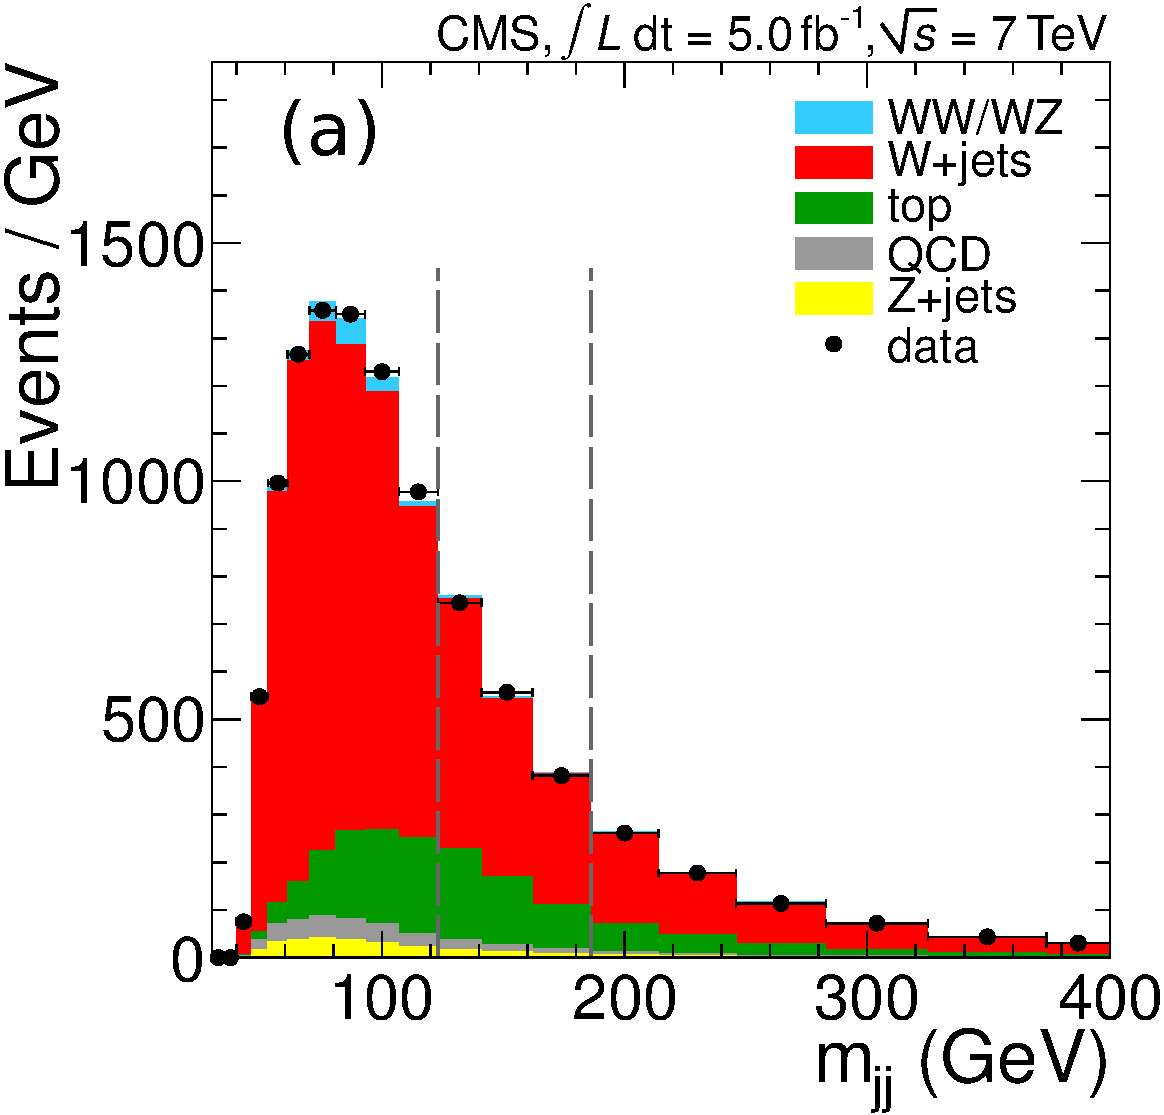
\includegraphics[width=\tripleColFig]{figs/Mjj_Stacked_combined.pdf}
  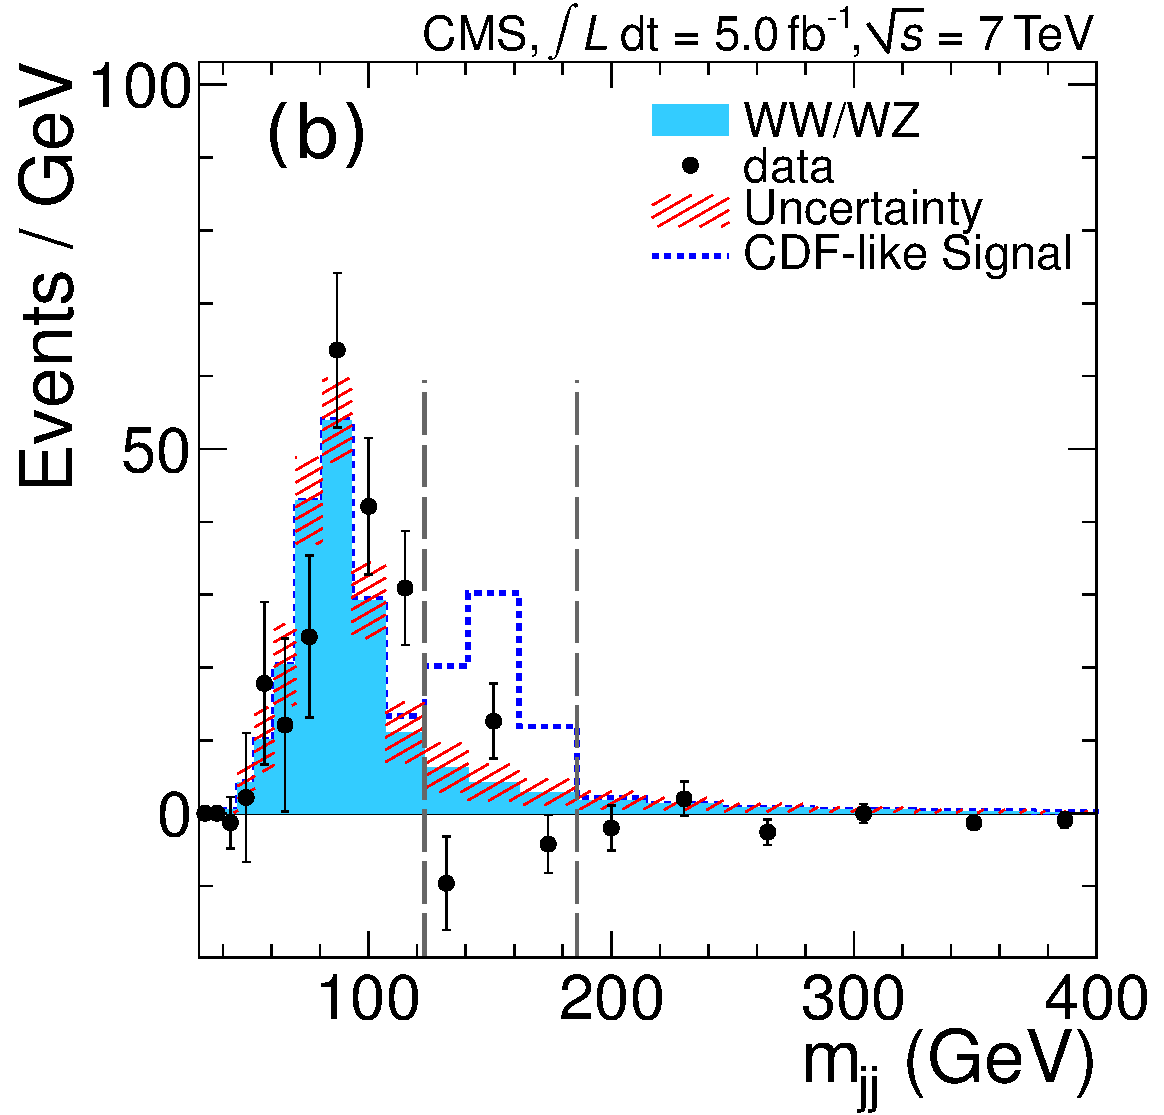
\includegraphics[width=\tripleColFig]{figs/Mjj_Subtracted_combined.pdf}
  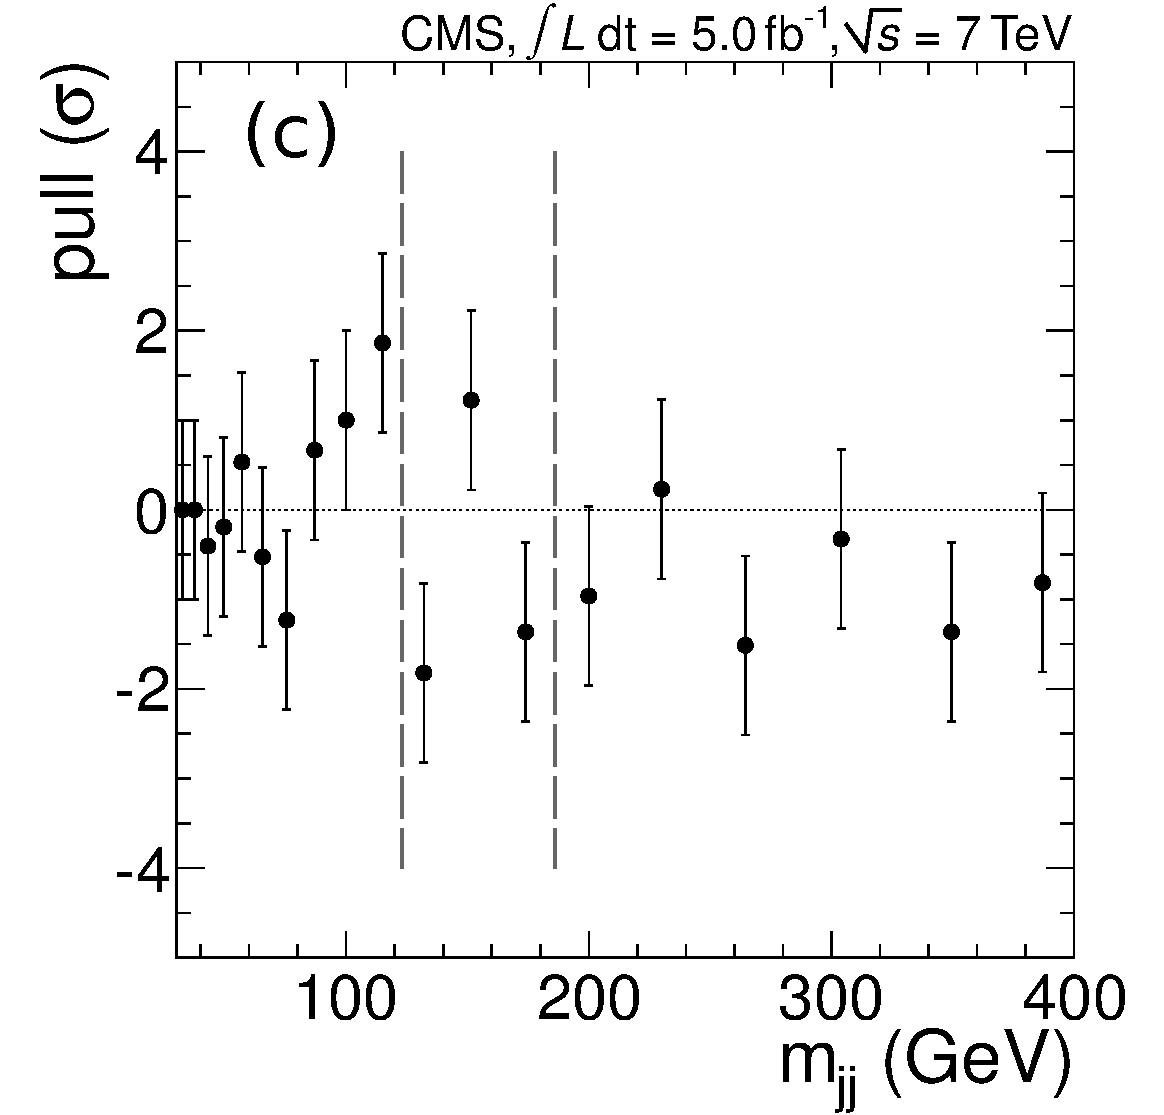
\includegraphics[width=\tripleColFig]{figs/Mjj_Pull_combined.pdf}
  \caption{(a) Distribution of the invariant mass spectrum of the
    leading two jets observed in data. Overlaid are the fit
    projections of the various components.  The region between the
    vertical dashed lines is excluded from the fit.  Depicted is the
    number of events per GeV.  (b)~The same
    distribution after subtraction of all SM components except the
    electroweak processes \PW\PW/\PW\Z. Error bars correspond to the
    statistical uncertainties.  The hatched band represents the systematic
    uncertainty on the sum of the SM components.  (c)~The normalized
    residual, $(\text{data} - \text{fit})/(\text{fit uncertainty})$.}
    \label{fig:Fig1}
  \ifthenelse{\boolean{cms@external}}{%
  }
  {%
    \end{center}
  }
\end{figure*}

\begin{table*}[htbp]
  \caption{Event yields determined from maximum-likelihood fits to the data.
    The total fit yields are corrected for bias.
    The total fit uncertainties include the corrections derived from the fit 
    validation described in the text and the effect of correlations among the 
    individual contributions.  }
  \label{tab:yields}
\begin{ruledtabular}
  \begin{tabular} {lcccc}
                        & \multicolumn{2}{c}{muons}  & \multicolumn{2}{c}{electrons} \\
   Process              & 2-jet         & 3-jet       & 2-jet          & 3-jet \\
\hline
   \Wpj               & $58919 \pm 530$ & $13069 \pm 366$ & $29787 \pm 1153$ & $\phantom{0}8397 \pm 292$ \\
   Dibosons             & $\phantom{0}1236 \pm 114$  & $\phantom{00}333 \pm 32\phantom{0}$    & $\phantom{00}685 \pm 65\phantom{00}$     & $\phantom{00}184 \pm 18\phantom{0}$ \\
   \ttbar               & $\phantom{0}4570 \pm 307$  & $\phantom{0}9049 \pm 382$  & $\phantom{0}2556 \pm 174\phantom{0}$   & $\phantom{0}4265 \pm 253$ \\
   Single-top           & $\phantom{0}1765 \pm 87\phantom{0}$   & $\phantom{0}1001 \pm 50\phantom{0}$   & $\phantom{00}916 \pm 46\phantom{00}$     & $\phantom{00}521 \pm 26\phantom{0}$ \\
   Drell--Yan plus jets & $\phantom{0}1837 \pm 79\phantom{0}$   & $\phantom{00}561 \pm 24\phantom{0}$    & $\phantom{0}1061 \pm 46\phantom{00}$    & $\phantom{00}364 \pm 16\phantom{0}$ \\
   Multijet (QCD)       & $\phantom{000}29 \pm 284$    & $\phantom{0000}0 \pm 90\phantom{0}$      & $\phantom{0}3944 \pm 1133$  & $\phantom{00}324 \pm 160$ \\
\hline
  Fit $\chi^2$ probability&   0.454      & 0.729           & 0.969            & 0.991 \\
   Total from fit       & $68294 \pm 307$ & $24013 \pm 193$ & $38949 \pm 228\phantom{0}$  & $14055 \pm 143$ \\
   Data                 & 67900           & 24046           & 38973            & 14145 \\
\hline
\hline
\multicolumn{5}{c}{In the signal region $123 < m_{jj} < 186\GeV$ (excluded from the fit)} \\
\hline
   Total predicted      & $14511 \pm 125$ & $\phantom{0}7739 \pm 95\phantom{0}$   & $\phantom{0}7944 \pm 92\phantom{00}$    & $\phantom{0}4347 \pm 70\phantom{0}$ \\
   Data                 & 14050           & 7751            & 8023             & 4438 \\
  \end{tabular}
\end{ruledtabular}
\end{table*}

Figure~\ref{fig:Fig1}(a) shows the observed \mjj distribution for all
four event categories combined, together with the fitted projections of the
contributions of various SM processes.  Figure~\ref{fig:Fig1}(b) shows
the same distribution after subtraction of all SM contributions from
data except electroweak diboson \PW\PW/\PW\PZ\ events.  No peak is visible in
the spectrum except that near 80\GeV due to diboson events.
Figure~\ref{fig:Fig1}(c) shows the normalized residuals.
Table~\ref{tab:yields} presents the yields of various SM components
obtained from the fit.  The sum of all the contributions is compared
to the number of observed events.  All numbers except those in the last
two rows are for the \mjj range of 40 to 400\GeV.  The last two rows
compare the observed and predicted contributions in the \mjj range of
123 to 186\GeV.  The data agree with the SM expectations, and we find
no significant excess in the signal region. We observe a sizable deficit
in the muon 2-jet data with respect to the prediction from our model.
We do not observe similar deviations in the other three categories,
suggesting it is a fluctuation and not a systematic bias.


%\section{Fit validation and systematic error estimate}

We validate the fit procedure by performing pseudo-experiments.  In
each experiment, we generate the \mjj pseudo-data of the SM processes,
taking into account the correlation among the yields, and then fit
each pseudo-data sample.  The results indicate that the bias on the
total yield is below 0.2\% and that the fit underestimates the total
yield uncertainty by about 30\%.  These effects are corrected for in
the final result.  Uncertainties in the jet energy are estimated using
a sample of \PW\ bosons decaying hadronically in a pure sample of
semileptonic \ttbar\ events.  The mean and resolution of the
reconstructed dijet mass distribution in data agree within 0.6\% with
the expectation from simulation.  A small difference in \met
resolution~\cite{Chatrchyan:2011tn} between data and simulation
affects the signal acceptance for the new physics models under
consideration at the 0.5\% level.  Further systematic uncertainties
are due to the uncertainty of the trigger efficiency estimates (1\%)
and the estimate of lepton reconstruction and selection efficiency
(2\%)~\cite{WZCMS:2010}.  The uncertainty on the integrated luminosity
is 2.2\%~\cite{lumiPAS}.
 
%\section{Results on presence of possible resonant enhancement}

We scrutinize the dijet mass spectrum near 150\GeV, searching for a
technicolor, leptophobic $\zp$, or \PW\PH\ resonant enhancement.  We also
use a generic signal model obtained by convolving a delta function
centered at $\mjj=150\GeV$ with a Gaussian function having width equal
to $\sigma_{jj}$.  The expected number of signal events at the LHC 
for a given cross section at the Tevatron can be
estimated by considering the ratio of the predicted cross sections for
our reference process, \PW\PH\ production with $M_{\text{H}} = 150\GeV$.
This process is dominated by quark-antiquark (\cPq\cPaq) annihilation.
As \cPq\cPaq\ processes have the smallest increase in parton
luminosity from the Tevatron to the LHC, this choice provides a
conservative limit.  We therefore assume
\begin{linenomath}
\begin{equation}
\sigma_{\text{LHC}}^{\text{dijet resonance}} = 
\sigma_{\text{Tevatron}}^{\text{dijet resonance}}  
\frac{\sigma_{\text{LHC}}^{\PW\PH}}{\sigma_{\text{Tevatron}}^{\PW\PH}},\label{eqTevToLHC2}\nonumber
\end{equation}
\end{linenomath}
where $\sigma_{\text{LHC}}^{\PW\PH} =
300.1\unit{fb}$~\cite{LHC4PDFxsec} and
$\sigma_{\text{Tevatron}}^{\PW\PH} =
71.8\unit{fb}$~\cite{Carena:2000yx}.  A generic Gaussian signal
normalized to $\sigma_{\text{Tevatron}} = 4\unit{pb}$ corresponds to
$\sigma_{\text{LHC}} = 16.7\unit{pb}$.  The values of
$\sigma_{\text{LHC}}\times \mathcal{B}(X\rightarrow jj)$ and
$\varepsilon\mathcal{A}$ for the models considered are given in
Table~\ref{tab:signals}.
% The expected yield is then
% \begin{linenomath}
%   \begin{equation}
%     N^{\text{signal}} = \sigma_{\text{LHC}}^{\text{dijet resonance}} \cdot 
%     \mathcal{B}(\PW\to\ell\nu) 
%     \cdot (\varepsilon\mathcal{A}) 
%     \cdot \int \mathcal{L}\ \text{d}t, 
%     \label{eqTevToLHC}
%     \nonumber
%   \end{equation}
% \end{linenomath}
% where $\mathcal{B}(\PW\to\ell\nu) = 0.2132$~\cite{pdg} for $\ell \in
% \left\{\Pe,\mu \right\}$, $\varepsilon\mathcal{A}$ denotes
% $\text{efficiency} \times \text{acceptance}$ for \PW\PH\ events, and
% $\int \mathcal{L}\ \text{d}t = 5.0\fbinv$ is the integrated
% luminosity.


\begin{table}[btph]
  \caption{\label{tab:signals} The {\sc pythia} cross 
    sections at 7~TeV times branching fraction to jets 
    ($\sigma\times\mathcal{B}$) and
    overall efficiency times acceptance ($\varepsilon\mathcal{A}$) for
    various signal models.  The relative uncertainties in $\varepsilon$ 
    measurements are 1--2\%.}
\begin{ruledtabular}
  \begin{tabular}{l c c c c c}
    &   & \multicolumn{4}{c}{$\varepsilon\mathcal{A}$} \\
    &   & \multicolumn{2}{c}{muons} & \multicolumn{2}{c}{electrons} \\
    Signal model &  $\sigma\times\mathcal{B}$ (pb) & 2-jet & 3-jet & 2-jet & 3-jet \\
    \hline
    Technicolor~\cite{Eichten:2011sh} & 7.4   & 0.065 & 0.020 & 0.039 & 0.011 \\
    $\zp$~\cite{Buckley:2011vc}       & 8.1   & 0.070 & 0.023 & 0.042 & 0.014 \\
    \PW\PH~\cite{Sjostrand:2006za}    & 0.059 & 0.060 & 0.019 & 0.038 & 0.013 \\
  \end{tabular}
\end{ruledtabular}
\end{table}

\begin{figure}[btph]
  \ifthenelse{\boolean{cms@external}}{%
  }
  {%
    \begin{center}
  }
%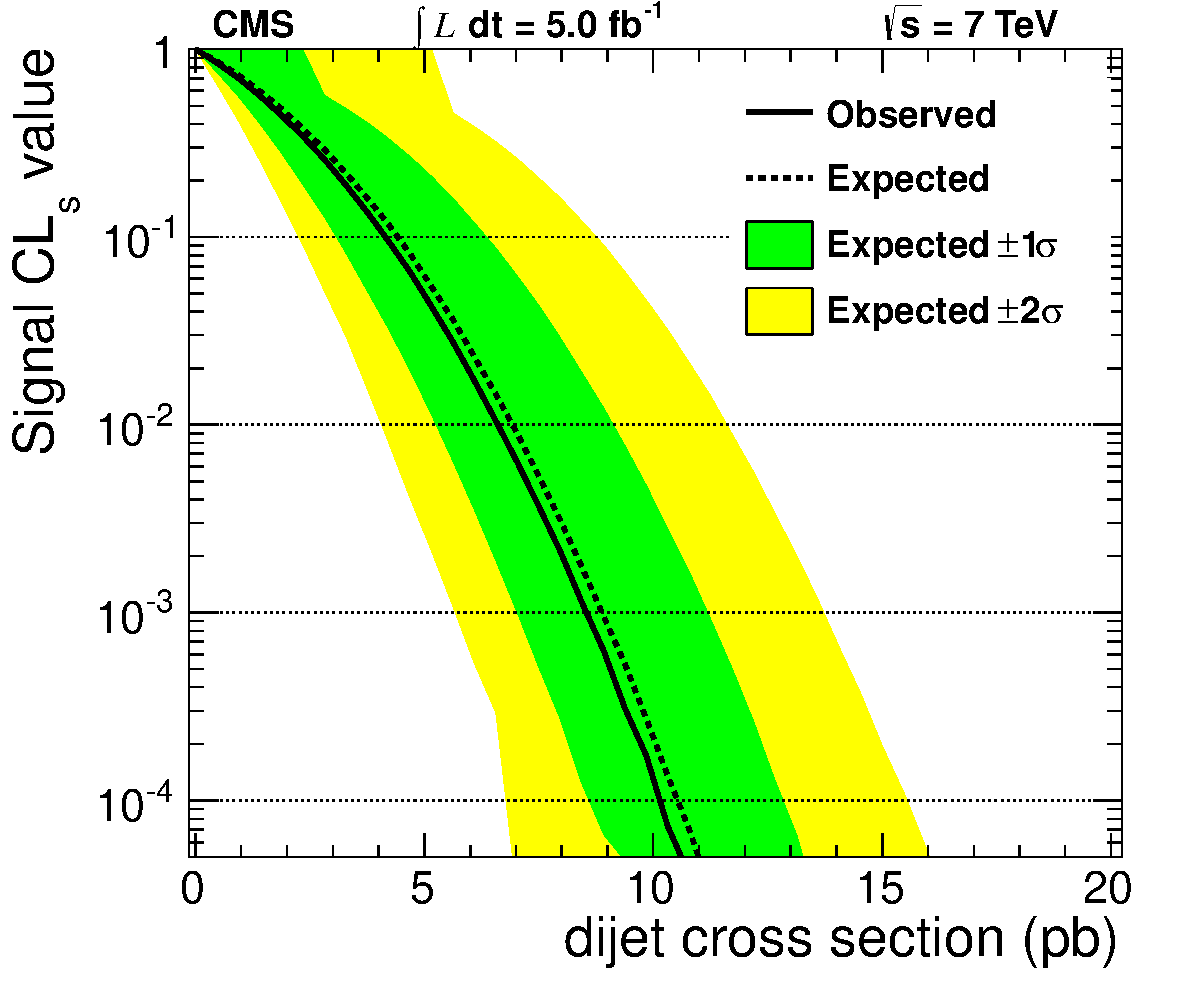
\includegraphics[width=0.4\textwidth]{figs/mjjpvalues.pdf}
%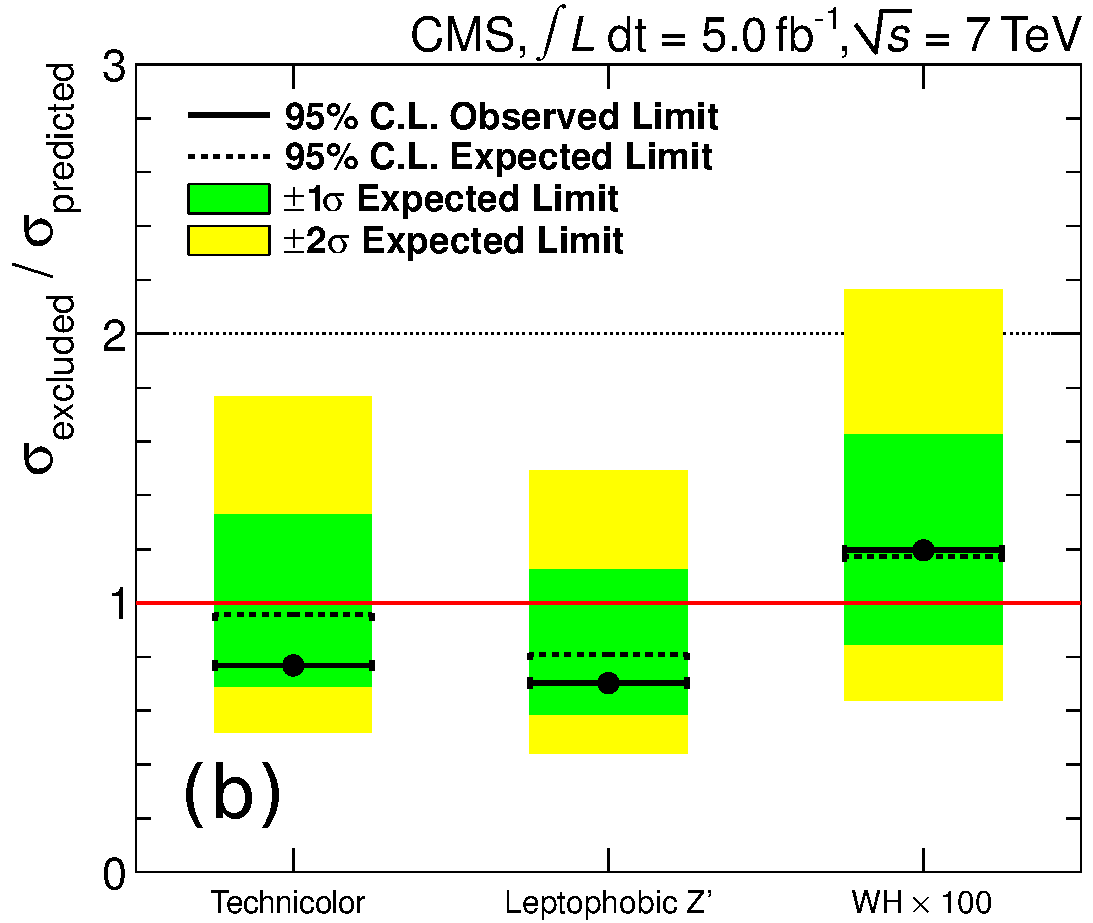
\includegraphics[width=0.4\textwidth]{figs/mjjlimitbars.pdf}
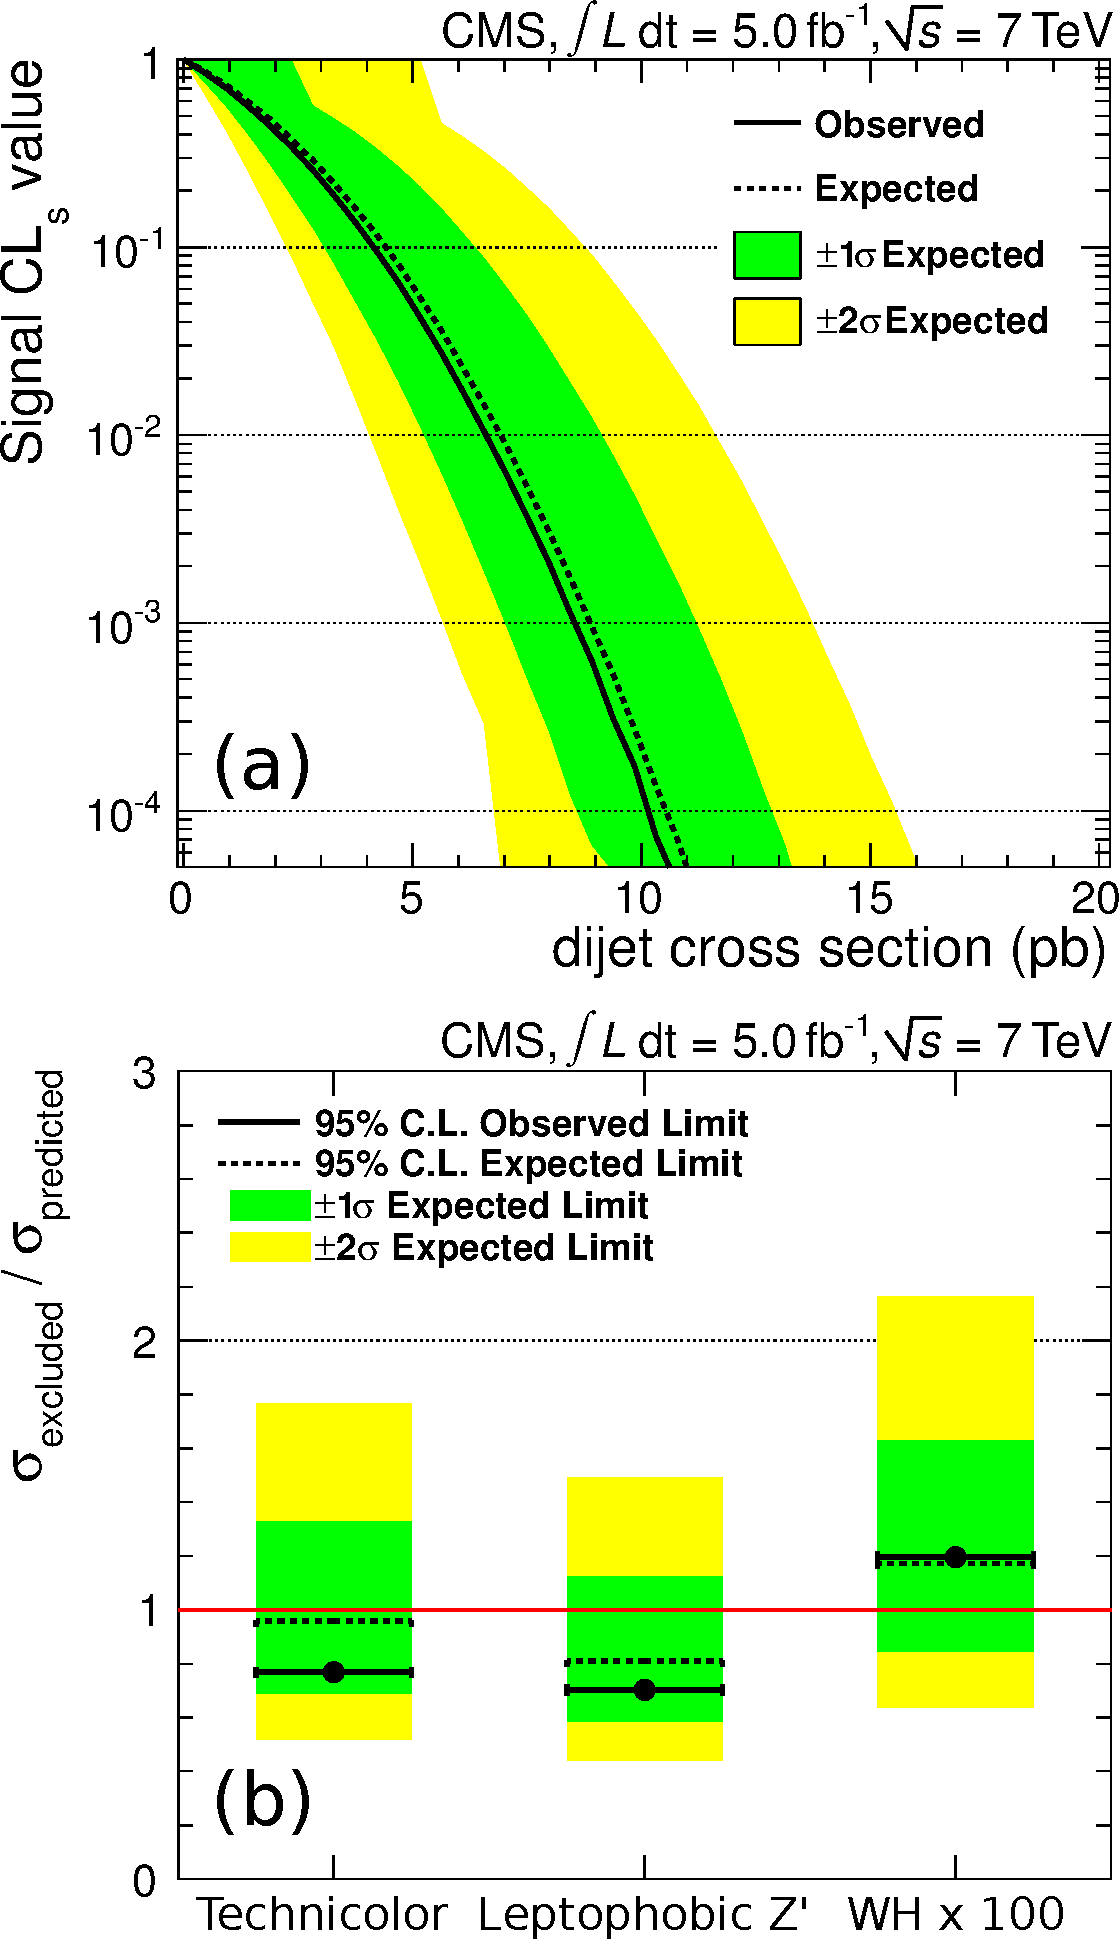
\includegraphics[width=\columnfigure]{figs/mjjlimits.pdf}
\caption{\label{fig:Fig2}(a) The observed and expected values of the
  $\text{CL}_{\text{S}}$ statistic for a generic Gaussian signal
  hypothesis with $M=150\GeV$ and $\sigma=15\GeV$, as a function of the 
  dijet signal cross section.
  (b)~Observed and expected 95\% CL upper limits, with one- and two-sigma 
  error bands, on the cross section divided by the expected values
  for various signal models. 
  The limits are calculated using the $\text{CL}_{\text{S}}$
  method. A value of the excluded cross section over the predicted
  cross section of less than one indicates that the model is excluded
  at 95\% CL.  Table~\ref{tab:signals} lists the cross sections for
  these models.  }
  \ifthenelse{\boolean{cms@external}}{%
  }
  {%
    \end{center}
  }
\end{figure}
%%%%%%%%%%%%%%%%%%%

Since we observe no resonant enhancement, we proceed to set exclusion
limits using a modified frequentist $\text{CL}_{\text{S}}$
method~\cite{CLS,Junk:1999kv} with profile likelihood as the test
statistic.  Inputs to the limit-setting procedure are the \mjj
distribution obtained by combining the SM components from the fit, the
observed distribution in data, and the expectation from the dijet
resonance model under consideration.  Figure~\ref{fig:Fig2}(a) shows
the observed and expected $\text{CL}_{\text{S}}$ values versus cross
section for a generic Gaussian signal, after combining the results of
all four event categories.  We set a 95\% confidence level (CL) upper
limit of 5.0\unit{pb} and a 99.9\% CL upper limit of 8.5\unit{pb} on
the dijet production cross section for a generic resonance with
\PW\PH-like $\varepsilon\mathcal{A}$.

Figure~\ref{fig:Fig2}(b) compares the 95\% CL upper limits with the
expected cross sections for technicolor, leptophobic $\zp$, and \PW\PH
($M_{\text{H}} = 150\GeV$) signals.  The technicolor and $\zp$ models
are excluded. Because we have minimal sensitivity to \PW\PH, we compare
the limit in Fig.~\ref{fig:Fig2}(b) to 100 times the SM
cross section as an illustration.

In summary, we have studied the invariant mass spectrum of the two
jets with highest transverse momentum in
$\text{pp}\rightarrow\PW$+2-jet and \PW+3-jet events, with the \PW\
decaying leptonically to a muon or electron.  The analyzed data sample
corresponds to an integrated luminosity of 5.0\fbinv at $\sqrt{s} =
7\TeV$.  We find no evidence for a resonant enhancement near a dijet
mass of 150\GeV, as reported by the CDF Collaboration, and set upper
limits on the dijet production cross section of 5.0\unit{pb} at 95\%
CL and 8.5\unit{pb} at 99.9\% CL.  Two theoretical models, leptophobic
$\zp$ and technicolor, which predict the presence of a resonant
enhancement near 150\GeV, are excluded.

% >> acknowledgements (for journal papers)
% Please include the latest version from https://twiki.cern.ch/twiki/bin/viewauth/CMS/Internal/PubAcknow.
%\section*{Acknowledgements}
We thank Adam Martin and Matthew Buckley for help with simulation of
technicolor and \zp models, respectively.  We congratulate our
colleagues in the CERN accelerator departments for the excellent
performance of the LHC machine. We thank the technical and
administrative staff at CERN and other CMS institutes, and acknowledge
support from FMSR (Austria); FNRS and FWO (Belgium); CNPq, CAPES,
FAPERJ, and FAPESP (Brazil); MES (Bulgaria); CERN; CAS, MoST, and NSFC
(China); COLCIENCIAS (Colombia); MSES (Croatia); RPF (Cyprus); MoER,
SF0690030s09 and ERDF (Estonia); Academy of Finland, MEC, and HIP
(Finland); CEA and CNRS/IN2P3 (France); BMBF, DFG, and HGF (Germany);
GSRT (Greece); OTKA and NKTH (Hungary); DAE and DST (India); IPM
(Iran); SFI (Ireland); INFN (Italy); NRF and WCU (Korea); LAS
(Lithuania); CINVESTAV, CONACYT, SEP, and UASLP-FAI (Mexico); MSI (New
Zealand); PAEC (Pakistan); MSHE and NSC (Poland); FCT (Portugal); JINR
(Armenia, Belarus, Georgia, Ukraine, Uzbekistan); MON, RosAtom, RAS
and RFBR (Russia); MSTD (Serbia); MICINN and CPAN (Spain); Swiss
Funding Agencies (Switzerland); NSC (Taipei); TUBITAK and TAEK
(Turkey); STFC (United Kingdom); DOE and NSF (USA).

